\section{Results and discussion}
\label{sec:results}

\subsection{Overview of the campaign}
\label{subsec:overview}

The campaign comprises $24$ converged simulations at $N=384$: three Reynolds numbers ($Re=100$, $400$ and $1000$), the full exponent sequence ($n=2$, $4$, $6$ and $8$) at each of them, and the two amplitudes $\alpha=0$ and $0.1$. Additional runs at $N=128$ and $N=256$ provide the resolution-sensitivity data of Section~\ref{subsec:resolution}. All $N=384$ simulations met the iterative criterion with final relative velocity changes at or below $9.9\times10^{-9}$. The complete scalar dataset is tabulated in the supplementary material; only the cases that support the argument are discussed here.

\subsection{Representative flow fields}
\label{subsec:fields}

Figure~\ref{fig:fields} presents the velocity-magnitude streamlines at $Re=400$, $N=384$ for all eight combinations $(n,\alpha)\in\{2,4,6,8\}\times\{0,0.1\}$ on a common color scale (colorbar in Fig.~\ref{fig:fields}). Two representative levels are shown because the full exponent sequence is now available at all three Reynolds numbers and $Re=400$ is the intermediate one, and because the undulated wall ($\alpha=0.1$) clears a larger portion of the cavity than the flat one; presenting both in the same figure avoids reporting the flat-wall fields in isolation. In all eight panels the lid drives a single dominant recirculation cell whose centre stays close to the cavity centre. The undulation produces a weak secondary structure attached to the bottom trough and a slightly more distorted near-wall shear layer, whereas increasing $n$ mainly flattens the bottom contour and removes the near-corner fillet. The change from $n=2$ to $n=4$ is the largest single geometric step; for $n=6$ and $n=8$ the streamline patterns at a given amplitude become nearly indistinguishable. These images are qualitative only: the quantitative energetic response, including the amplitude interaction, is given in Figs.~\ref{fig:energetic} and~\ref{fig:contrasts}. Complete field maps for every converged configuration, again separated by amplitude, are compiled in the supplementary material (Figs.~SM.2 and SM.3).

\begin{figure}[t]
\centering
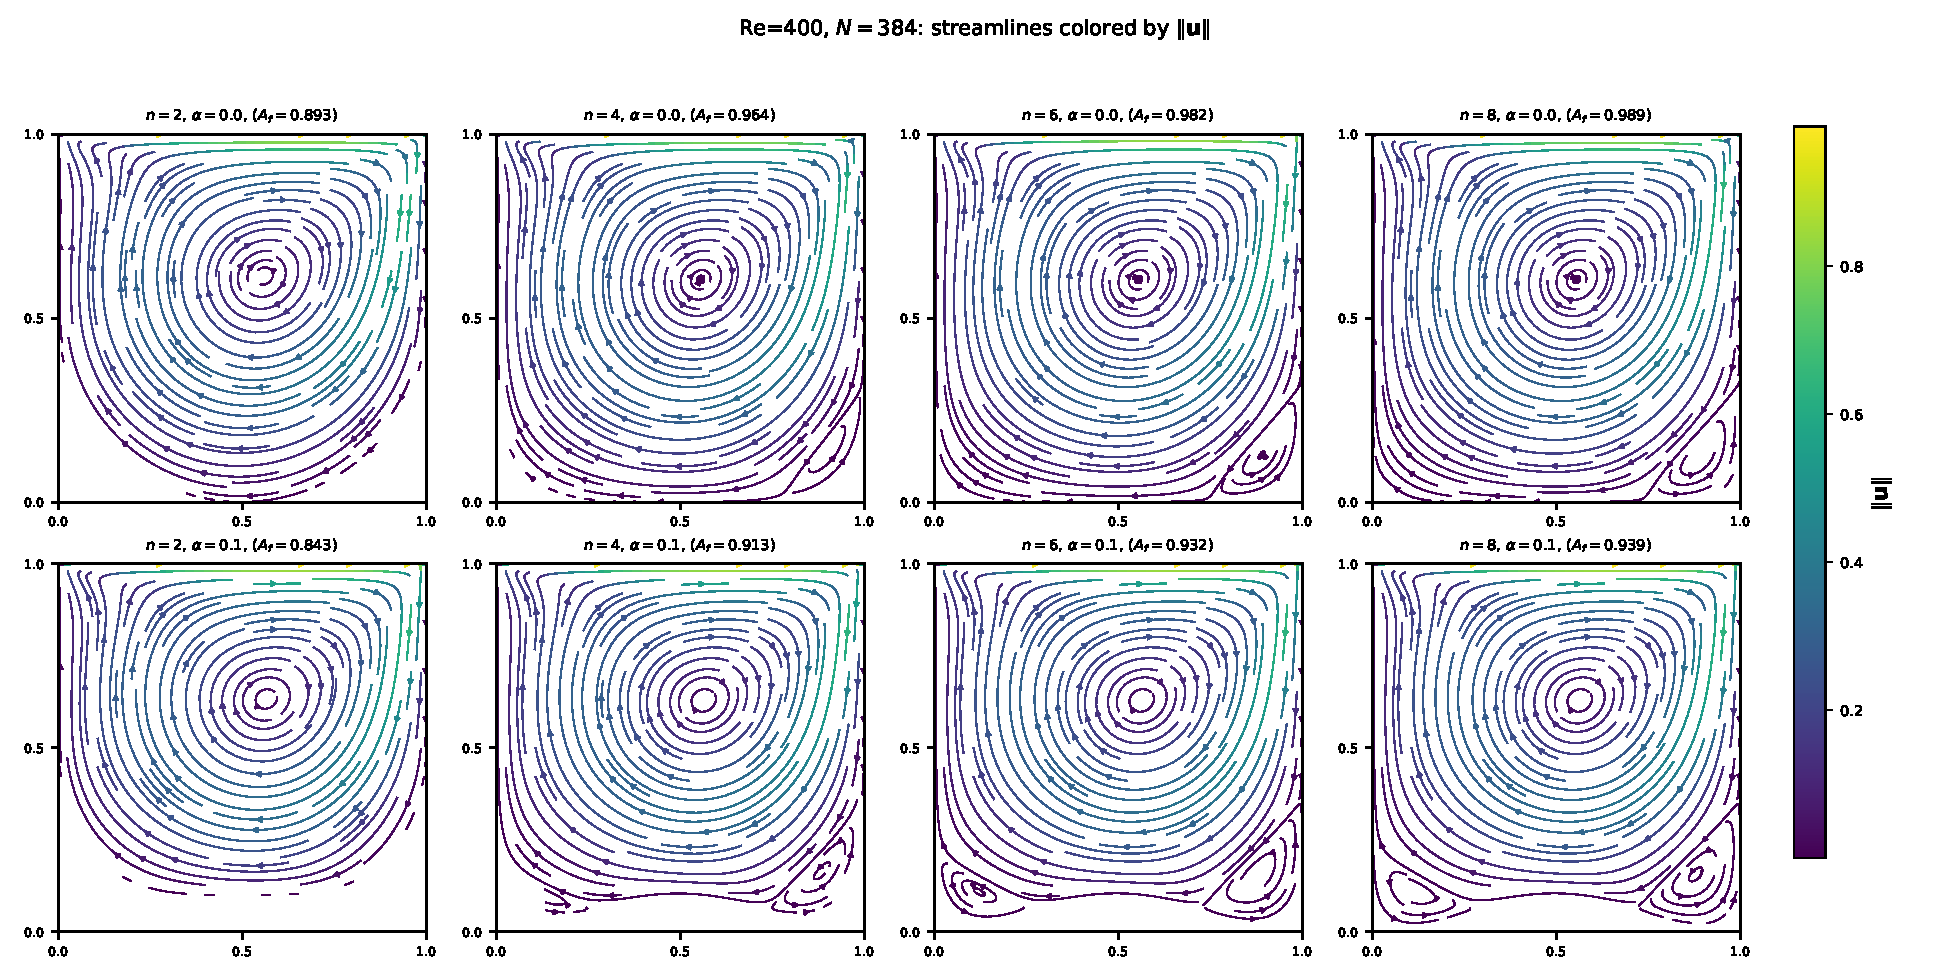
\includegraphics[width=0.98\columnwidth]{figures/fig3_fields.pdf}
\caption{(Color online) Streamlines colored by velocity magnitude at $Re=400$, $N=384$. Top row: $\alpha=0$ ($n=2$,$4$,$6$,$8$). Bottom row: $\alpha=0.1$ ($n=2$,$4$,$6$,$8$). Panels labeled by $(n,\alpha)$ with fluid area $A_f$. All panels share a common color scale $\|\mathbf{u}\|$ as indicated; the inclusion of both amplitudes allows a direct qualitative comparison between undulated and non-undulated cavities for each exponent.}
\label{fig:fields}
\end{figure}

\subsection{Spatial origin of the geometric contrast}
\label{subsec:mechanism}

The global integrals show \emph{that} the dissipation responds weakly to the bottom geometry; we now localize \emph{where} the change occurs. Figure~\ref{fig:dissipation} shows the local dissipation density $2\mu\,\mathbf{S}{:}\mathbf{S}$ at $Re=400$, $\alpha=0$, for $n=2$ and $n=4$, together with their difference $\Delta(2\mu\mathbf{S}{:}\mathbf{S})$. The dissipation is overwhelmingly concentrated in the shear layer under the lid: integrating over horizontal bands, the top $10\%$ of the cavity contains $77.8\%$ of $D^*$ at $Re=400$ and the top $20\%$ contains about $90\%$; the bottom-wall band below $y_b+0.1$ holds only $1.0\%$ ($n=2$) and $0.4\%$ ($n=4$). This near-lid concentration is nearly a one-parameter function of $Re$, and it \emph{weakens} slowly with Reynolds number---the top-$10\%$ share falls from $83.7\%$ at $Re=100$ to $77.8\%$ at $Re=400$ and $74.3\%$ at $Re=1000$---because the core circulation thickens and spreads its dissipation over a larger fraction of the cavity as $Re$ increases. The lid layer nevertheless remains the dominant dissipative zone at all three Reynolds numbers.

The geometric contrast is therefore not a bottom-wall friction effect. To localize it exactly, we partition the $n=4$ fluid region into two disjoint parts: the \emph{common} region $A$, consisting of cells that are fluid for both $n=2$ and $n=4$, and the \emph{added} region $B$, consisting of cells that are fluid for $n=4$ but solid for $n=2$ (the shoulder zones uncovered by flattening the bowl into the near-square). Then $\Delta D$ splits, cell by cell, into a redistribution term over $A$ and an added-zone term over $B$,
\begin{equation}
\Delta D \;=\; \underbrace{\sum_{A}\big(\ell_4-\ell_2\big)}_{dA}\;+\;\underbrace{\sum_{B}\ell_4}_{dB},
\end{equation}
where $\ell$ is the local dissipation density times the cell area. Because $A$ and $B$ are disjoint and their union is exactly the $n=4$ region, this identity closes to machine precision; there is no residual partition ambiguity. Table~\ref{tab:layers} reports the two terms at the three Reynolds numbers, together with their sum, which reproduces the headline contrast $I_D$ (defined in Eq.~\ref{eq:contrast}) to within $10^{-5}$ of itself.

\begin{table}[t]
\centering
\caption{Exact partition of the geometric dissipation contrast $\Delta D$ at $\alpha=0$, $N=384$. All entries are in units of $10^{-4}D^*(2,0)$. $dA$ is the redistribution within the region common to both geometries (its four disjoint bands are listed in Table~SM.XIII of the Supplementary Material); $dB$ is the dissipation of the added region available only to $n=4$. The last two columns are the sum $dA+dB=\Delta D$ and the corresponding headline contrast $I_D(2,4)=100\,\Delta D/D^*(2,0)$. The identity closes to machine precision.}
\label{tab:layers}
\begin{tabular}{@{}lcccc@{}}
\hline
$Re$ & $dA$ (common) & $dB$ (added) & $\Delta D=dA+dB$ & $I_D$ [\%] \\
\hline
$100$  & $-4.81$ & $+6.99$ & $+2.18$ & $+0.0218$ \\
$400$  & $+12.78$ & $+19.71$ & $+32.49$ & $+0.3249$ \\
$1000$ & $+10.44$ & $+48.65$ & $+59.09$ & $+0.5909$ \\
\hline
\end{tabular}
\end{table}

Two robust facts follow. First, the \emph{added} region always makes a positive contribution $dB$: uncovering the shoulder zones adds dissipation, and this term grows monotonically with Reynolds number, from $+6.99\times10^{-4}$ at $Re=100$ to $+4.87\times10^{-3}$ at $Re=1000$ (in units of $D^*(2,0)$). Crucially, the added region is weakly dissipative: it covers about $7.4\%$ of the total fluid area at $Re=400$ yet contributes only $0.20\%$ of $D^*$, so its mean dissipation density is about $2.7\%$ of the cavity average (about $1\%$ at $Re=100$ and $7\%$ at $Re=1000$). This is the most direct explanation of the sub-extensive response: the fluid added by flattening sits in a slow, weakly sheared shoulder region and dissipates almost nothing. Second, the redistribution term $dA$ is a small difference of much larger, opposing contributions from the four disjoint bands of the common region (Table~SM.XIII of the Supplementary Material): at $Re=400$ the lid band ($y>0.9$) contributes $+2.44\times10^{-3}$ and the interior core contributes $-2.83\times10^{-3}$, whose near-cancellation plus the bottom ($+6.21\times10^{-4}$) and side/corner ($+1.04\times10^{-3}$) bands leaves the small $dA=+1.28\times10^{-3}$; at $Re=1000$ the lid band is $+5.55\times10^{-3}$ and the core $-6.60\times10^{-3}$. The redistribution term $dA$ is negative only at $Re=100$ ($-4.81\times10^{-4}$) and changes sign near $Re\approx145$, as the low-$Re$ corner-dominated balance tips toward the lid-dominated one; the added-zone term $dB$ never changes sign. Note that $dA$ and $dB$ are \emph{not} of opposite sign at $Re\ge400$---both are positive---so the smallness of the net contrast is due to the near-cancellation \emph{inside} $dA$ (between the lid and core bands), not to a cancellation between $dA$ and $dB$. The mechanism is thus a competition between an always-positive but weakly dissipative added region and a common-region redistribution that is itself a near-cancellation of opposing band contributions.

The grid robustness of this mechanism is assessed in Table~SM.XV and Fig.~SM.5 of the Supplementary Material, where all four bands are recomputed cell by cell with the identical exact-partition code at every resolution $N=128$, $256$, $384$, and $512$ (the $N=384$ rows reproduce the headline partition to machine precision, and $N=512$ is available at $Re=400$ and $1000$). The cancellation index $C=\sum|\text{bands}|/|dA|$ grows both with Reynolds number and with refinement: about $4.0$ at $Re=100$, $5.0\to5.4$ at $Re=400$, and $11.3\to14.3$ at $Re=1000$ from $N=128$ to $N=512$, reflecting the increasing internal cancellation within $dA$ as the lid and core bands become larger and more opposed. Despite this, the net contrast $\Delta D = dA + dB$, which equals $I_D(2,4)$, remains stable to within $2.4\%$ of its value across $N=128$--$512$ at all three Reynolds numbers, because the grid-induced changes in $dA$ and $dB$ partially cancel. The sign and order of magnitude of $dA$ and $dB$ are therefore robust on every grid; their individual magnitudes carry a grid sensitivity that rises with $Re$ (the $dA$ span is $1.9\%$ of its value at $Re=100$, $8.2\%$ at $Re=400$ and $27\%$ at $Re=1000$), which is the price of the internal cancellation but does not contaminate the net contrast.

\begin{figure}[t]
\centering
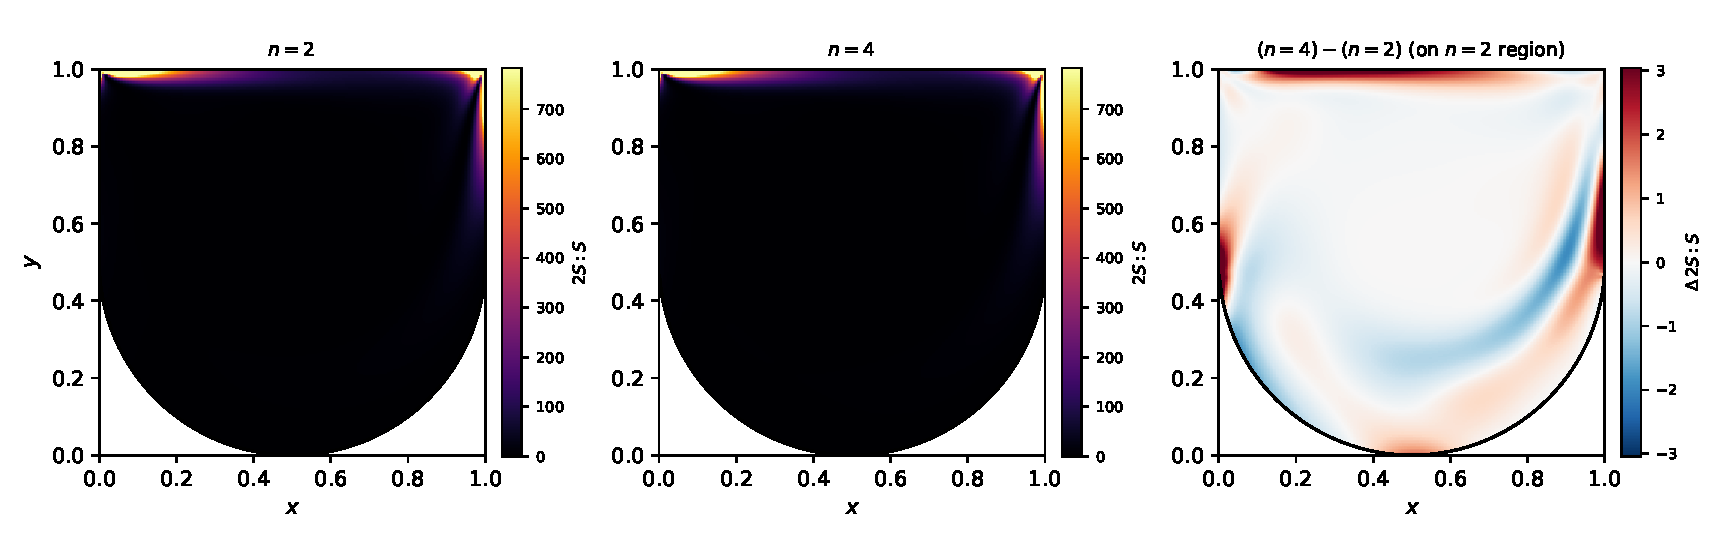
\includegraphics[width=0.98\columnwidth]{figures/fig7_dissipation_map.pdf}
\caption{(Color online) Local dissipation density $2\mu\,\mathbf{S}{:}\mathbf{S}$ at $Re=400$, $\alpha=0$, $N=384$: (left) $n=2$; (middle) $n=4$; (right) the difference $(n{=}4)-(n{=}2)$ evaluated on the $n=2$ fluid region. The dissipation is concentrated in the lid shear layer; the geometric contrast arises from a positive contribution of the added shoulder region plus a common-region redistribution that is a near-cancellation of a positive lid-band change against a negative interior-core change (Table~\ref{tab:layers}).}
\label{fig:dissipation}
\end{figure}

\subsection{Absolute energetic response}
\label{subsec:absresponse}

Figure~\ref{fig:energetic} shows $P^*$, $D^*$, and $K^*$ versus $n$ at $N=384$ for $\alpha=0$ (solid) and $\alpha=0.1$ (dashed). Several features are common to all Reynolds numbers. The power input and the dissipation increase strongly with $Re$: at $n=2$, $\alpha=0$, $D^*$ rises from $17.92$ ($Re=100$) to $23.43$ ($Re=400$) and $31.54$ ($Re=1000$). At fixed $Re$, both $P^*$ and $D^*$ increase slightly with $n$. The kinetic energy behaves differently: although it changes very little in \emph{absolute} terms over the exponent range (its total variation is below $1\%$ of its own value, and its curves in Fig.~\ref{fig:energetic} are visibly flat), its \emph{relative} geometric contrast $I_K(2,4)$ is actually larger than $I_D(2,4)$: $+0.67\%$ versus $+0.022\%$ at $Re=100$ and $+0.77\%$ versus $+0.32\%$ at $Re=400$ (at $Re=1000$ the ordering reverses, $I_K=+0.53\%$ against $I_D=+0.59\%$). The weak curvature of the $K^*$ curves therefore does not mean that $K^*$ is insensitive to the geometry: flattening the bottom shifts the recirculation slightly, and the relative change of the stored kinetic energy is comparable to, or larger than, that of the dissipation. What is genuinely small is the change of $D^*$ \emph{relative to the change in fluid area}, which is the sub-extensivity discussed next.

The small magnitude of the change in $D^*$ with $n$ is the central observation. Between $n=2$ and $n=4$ at $\alpha=0$, the fluid area grows by $7.9\%$ (from $0.8927$ to $0.9635$), yet $D^*$ grows by only $0.022\%$ ($Re=100$), $0.325\%$ ($Re=400$), and $0.591\%$ ($Re=1000$). The dissipation is therefore strongly sub-extensive relative to the area-only null model: adding fluid by flattening the bottom does not add a proportional amount of viscous dissipation, but instead reduces the dissipation per unit fluid area by approximately $7\%$ (Section~\ref{subsec:arearesult}). The remaining transitions are even weaker: at $Re=400$ the change from $n=4$ to $n=6$ adds $0.013\%$, and from $n=6$ to $n=8$ essentially nothing ($6\times10^{-5}\%$). At $Re=1000$ the same two steps are $+0.0103\%$ and $-0.0037\%$: the trailing transition is no longer vanishing but slightly negative, a point taken up in Section~\ref{subsec:contrastresult}. At $Re=100$ they are $+0.00296\%$ and $+0.00042\%$. The absolute values for all cases are collected in the supplementary material.

\begin{figure}[t]
\centering
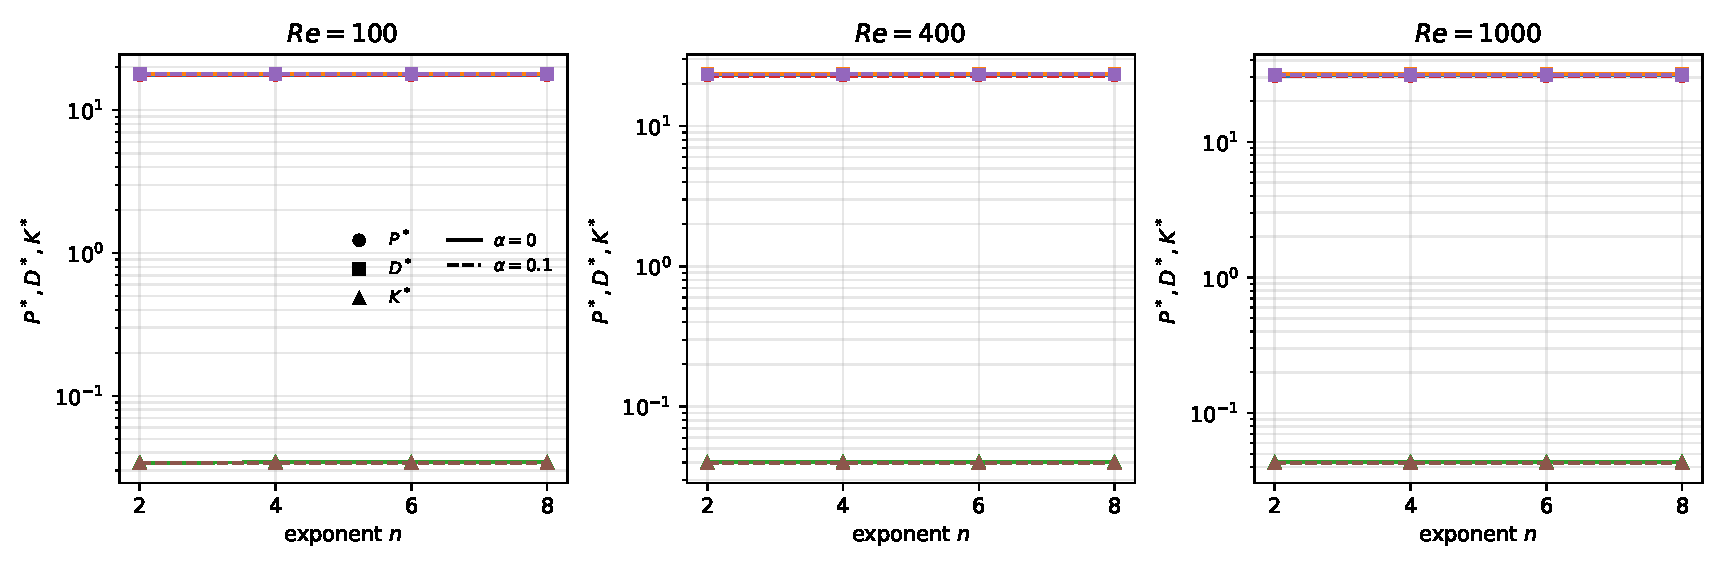
\includegraphics[width=0.95\columnwidth]{figures/fig4_energetic.pdf}
\caption{(Color online) Dimensionless energetic integrals versus superellipse exponent at $N=384$. Panels: (a) $Re=100$; (b) $Re=400$; (c) $Re=1000$. Solid lines: $\alpha=0$; dashed lines: $\alpha=0.1$. Circles: $P^*$; squares: $D^*$; triangles: $K^*$. The full sequence $n=2,4,6,8$ is available at all three Reynolds numbers. $P^*$ and $D^*$ vary strongly with $Re$ and weakly with $n$; $K^*$ is almost insensitive to $n$.}
\label{fig:energetic}
\end{figure}

\subsection{Test of the area-only extensive reference}
\label{subsec:arearesult}

Because $A_f$ increases with $n$, the extensive area reference of Eq.~\eqref{eq:area} is not identically zero. Figure~\ref{fig:contrasts} compares the measured contrasts $I_D$ and $I_P$ with $I_{D,\mathrm{area}}$ on a symmetric logarithmic ordinate: panel (a) resolves the three successive transitions at $Re=400$, and panel (b) the primary transition at the three Reynolds numbers. For the transition $(2,4)$ at $\alpha=0$, the extensive reference predicts $+7.93\%$, whereas the measured $I_D$ is $+0.022\%$ ($Re=100$), $+0.325\%$ ($Re=400$), and $+0.591\%$ ($Re=1000$). The measured and predicted contrasts share the same sign but differ in magnitude by factors of about $360$, $24$, and $13$, respectively. For $(4,6)$ the reference predicts $+1.91\%$ against a measured $+0.013\%$ at $Re=400$; for $(6,8)$ it predicts $+0.75\%$ against a measured $+6\times10^{-5}\%$ for $I_D$, while the power-based value is slightly negative ($I_P=-1.5\times10^{-4}\%$). 

The area-only model therefore does not explain the observations: it over-predicts the contrast, by factors of approximately $13$--$364$ across the Reynolds numbers studied. The correct reading is not that area is irrelevant---the area does change, and the dissipation does increase with $n$---but that the flow reorganizes so that the dissipation per unit fluid area decreases as the cavity is flattened. The area-only model is thus a simple extensive reference, not a quantitative prediction of the energetic response.

A sharper reference is the dissipation \emph{per unit fluid area}, $d^*=D^*/A_f$, which removes the trivial extensive part of the geometric change. At the primary transition this intrinsic density contrast, $I_{D/A}=100\,(d^*_4-d^*_2)/d^*_2$, is $-7.33\%$ ($Re=100$), $-7.05\%$ ($Re=400$), and $-6.80\%$ ($Re=1000$)---almost constant in $Re$ and strikingly close to the area-only prediction of $+7.93\%$ with the opposite sign. The area-only model sets the \emph{extensive} scale of the change; measured against that scale, the flow converts the added fluid into a proportionally \emph{lower} average dissipation rate. The per-area reference is therefore the physically meaningful baseline: it is $O(1)$ where the extensive reference over-predicts by factors of $13$--$364$. It should be read as a change of normalization rather than as an independent physical observable: when $I_D$ is small, $I_{D/A}$ is algebraically close to $-I_{D,\mathrm{area}}$, so its near-constant value of about $-7\%$ reflects the smallness of $I_D$ itself, not a separate physical mechanism. The physically independent information about the mechanism is carried by the $\mathrm{d}A/\mathrm{d}B$ partition of Section~\ref{subsec:mechanism} and Table~\ref{tab:layers}, not by the per-area normalization. The resolution-sensitivity analysis of Section~\ref{subsec:resolution} shows, however, that the per-area contrast inherits the residual grid error of the absolute area (the discrete mask area differs from the analytic area by at most $\sim0.02\%$ at $N=384$; see the area table of the supplementary material); we therefore quote both the extensive and per-area references and base no conclusion on their difference. Figure~\ref{fig:reference} summarizes the comparison.

\subsection{Matched geometric contrasts and their hierarchy}
\label{subsec:contrastresult}

Figure~\ref{fig:contrasts} and Table~\ref{tab:contrasts} summarize the successive contrasts. At $Re=400$, $\alpha=0$, the three measured dissipation contrasts are $I_D(2,4)=+0.3249\%$, $I_D(4,6)=+0.0129\%$, and $I_D(6,8)=+6\times10^{-5}\%$. The $(6,8)$ value is at or below its own $N = 128$--$384$ span ($1.1\times10^{-4}$~pp) and is quoted only as an upper bound; it is not resolved. Their shares of the sum of absolute magnitudes are approximately $96.2\%$, $3.8\%$, and $0.02\%$, respectively. These percentages are shares of the sum of the absolute magnitudes of the three successive contrasts; they are not fractions of a total energy budget. The same three-step sequence is now available at all three Reynolds numbers: $+0.0218\%$, $+0.00296\%$, $+0.00042\%$ at $Re=100$ and $+0.5909\%$, $+0.0103\%$, $-0.0037\%$ at $Re=1000$, i.e.\ shares of $86.6\%$, $11.8\%$, $1.7\%$ at $Re=100$ and $97.7\%$, $1.7\%$, $0.6\%$ at $Re=1000$. The concentration of the response in the $(2,4)$ transition is thus found at every Reynolds number studied, at very different absolute magnitudes.

At all three Reynolds numbers, for which the full exponent sequence is now available, the hierarchy $|I(2,4)|\gg|I(4,6)|\gg|I(6,8)|$ holds at both amplitudes examined (Section~\ref{subsec:amplitude}). It reflects the fact that the largest geometric change occurs at low $n$: the relief flattens most rapidly between $n=2$ and $n=4$, after which the cavity is already close to the square limit and further increases of $n$ alter the geometry only weakly. This is a statement about the range of exponents studied; it does not define a universal threshold at $n=4$ for other wall shapes or undulation counts.

At $Re=1000$, however, the trailing transitions do not vanish: $I_D(6,8)=-0.0037\%$ at $\alpha=0$, so beyond $n=4$ increasing the exponent slightly \emph{reduces} dissipation at the highest Reynolds number. This negative sign is resolved rather than marginal. The contrast is negative on all three grids ($-0.00371\%$, $-0.00360\%$, $-0.00371\%$ at $N=128$, $256$, $384$), with a span of $1.1\times10^{-4}$ percentage points, i.e.\ more than thirty times smaller than its own magnitude, and $(4,6)=+0.0103\%$ is likewise resolved by its own span of $4.1\times10^{-4}$ percentage points. At $Re=400$ the same $(6,8)$ transition changes sign between $N=128$ and $N=256$ and stays inside its span, so no sign can be assigned there. The $Re=1000$ value is therefore reported as the first resolved negative trailing step, not as a measured reversal from a demonstrated positive one. The undulation amplitude lowers the Reynolds number at which the trailing steps become negative: at $\alpha=0.1$ both are negative and already resolved at $Re=400$ ($-0.0039\%$ with a span of $8.7\times10^{-4}$~pp, and $-0.0017\%$ with a span of $8.5\times10^{-5}$~pp), and both stay negative at $Re=1000$ ($-0.0242\%$ and $-0.0052\%$). At $Re=100$ and $\alpha=0$ both trailing steps remain positive ($+0.00296\%$ and $+0.00042\%$); $(6,8)$ is stable across the three grids (span $8.1\times10^{-5}$~pp), whereas $(4,6)$ is not resolved at this Reynolds number, its $N=128$--$384$ span reaching $1.15$~pp because the coarse-grid $n\ge6$ cases reach a local Mach number of $0.18$ and their absolute dissipation is not comparable to the $n=4$ one there.

\begin{table}[t]
\centering
\caption{Matched dissipation and power contrasts at $N=384$, $\alpha=0$, expressed as percentages of the earlier configuration of each pair. The last three columns give the estimator discrepancy $\delta_{IP/ID}=100|I_P/I_D-1|$, the area-only extensive prediction, Eq.~\eqref{eq:area}, and the numerical uncertainty. Uncertainty is the span of the contrast itself over $N = 128$--$384$ at fixed ($Re$, transition). A contrast is treated as resolved when its magnitude exceeds its own span: this holds for every $(2,4)$ entry, for $(4,6)$ at $Re=400$ and $Re=1000$, and for $(6,8)$ at $Re=100$ and $Re=1000$, and fails for $(4,6)$ at $Re=100$ and $(6,8)$ at $Re=400$, which are therefore reported as upper bounds only (marked $\dagger$).}
\label{tab:contrasts}
\begin{tabular}{@{}ccccccc@{}}
\hline
$Re$ & Transition & $I_D$ [\%] & $I_P$ [\%] & $\delta_{IP/ID}$ [\%] & $I_{D,\mathrm{area}}$ [\%] & uncertainty [pp] \\
\hline
$100$  & $(2,4)$ & $+0.0218$ & $+0.0211$ & $3.1$  & $+7.93$ & $3.4\times 10^{-4}$ \\
$100$  & $(4,6)$ & $+0.00296$ & $+0.00264$ & $10.6$ & $+1.91$ & $1.15^{\dagger}$ \\
$100$  & $(6,8)$ & $+0.00042$ & $+0.00040$ & $4.5$  & $+0.75$ & $8.1\times 10^{-5}$ \\
$400$  & $(2,4)$ & $+0.3249$ & $+0.3282$ & $1.0$  & $+7.93$ & $2.4\times 10^{-3}$ \\
$400$  & $(4,6)$ & $+0.0129$ & $+0.0115$ & $10.3$ & $+1.91$ & $5.0\times 10^{-4}$ \\
$400$  & $(6,8)$ & $+0.00006$& $-0.00015$& --     & $+0.75$ & $1.1\times 10^{-4}$\,$^{\dagger}$ \\
$1000$ & $(2,4)$ & $+0.5909$ & $+0.6022$ & $1.9$  & $+7.93$ & $1.3\times 10^{-2}$ \\
$1000$ & $(4,6)$ & $+0.0103$ & $+0.0062$ & $40.4$ & $+1.91$ & $4.1\times 10^{-4}$ \\
$1000$ & $(6,8)$ & $-0.0037$ & $-0.0043$ & $15.6$ & $+0.75$ & $1.1\times 10^{-4}$ \\
\hline
\end{tabular}
\end{table}
\begin{figure}[t]
\centering
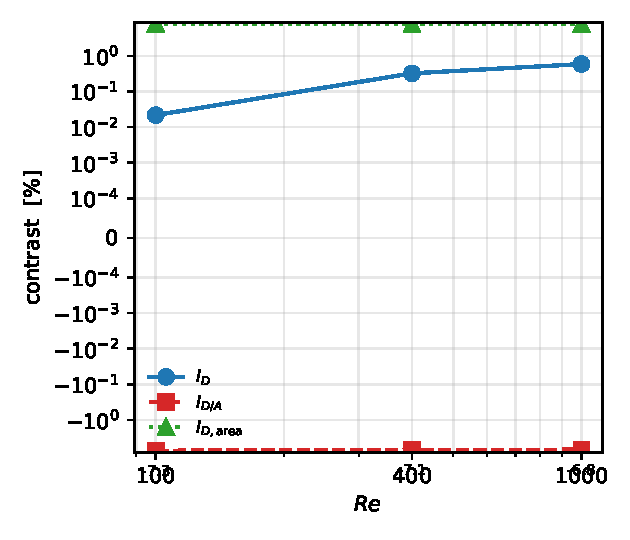
\includegraphics[width=0.6\columnwidth]{figures/fig8_reference.pdf}
\caption{(Color online) Primary transition $(2,4)$, $\alpha=0$, at $N=384$: measured dissipation contrast $I_D$ (circles), intrinsic contrast per unit fluid area $I_{D/A}$ (squares), and the extensive area-only reference $I_{D,\mathrm{area}}$ (triangles), on a symmetric logarithmic ordinate. The extensive reference lies a factor of about $24$ above the measurement, whereas the per-area contrast is the same order of magnitude with the opposite sign. The per-area curve is shown as a change of normalization, not as independent physical evidence; for small $I_D$ it is algebraically close to $-I_{D,\mathrm{area}}$.}
\label{fig:reference}
\end{figure}
\begin{figure}[t]
\centering
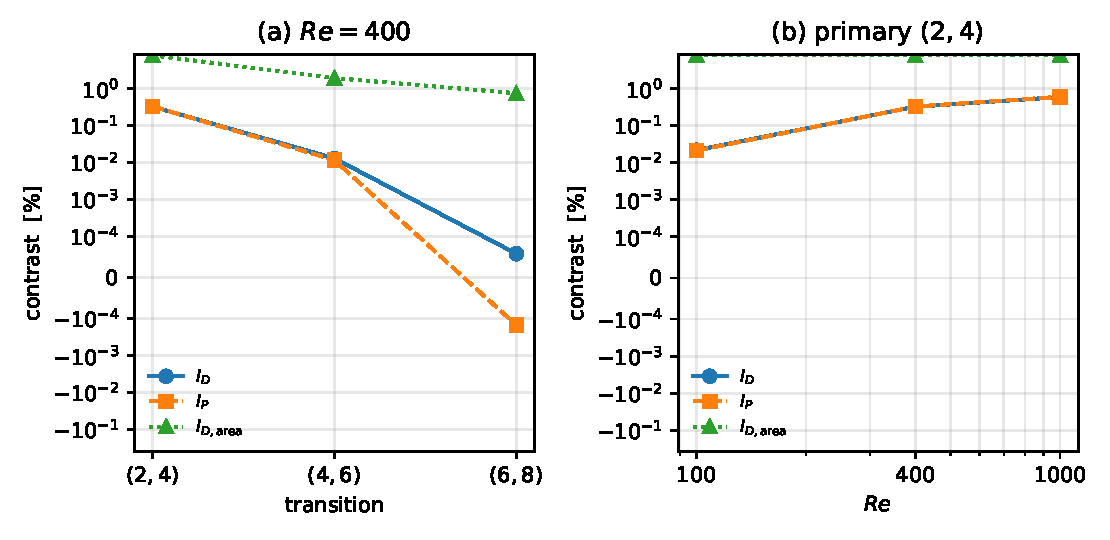
\includegraphics[width=0.95\columnwidth]{figures/fig5_contrasts.pdf}
\caption{(Color online) Matched contrasts at $N=384$, $\alpha=0$, on a symmetric logarithmic ordinate. (a) $Re=400$: the three successive transitions $(2,4)$, $(4,6)$, $(6,8)$, with dissipation $I_D$ (circles), power $I_P$ (squares), and the area-only extensive prediction $I_{D,\mathrm{area}}$ (triangles). (b) Primary transition $(2,4)$ at $Re=100$, $400$, $1000$. Every coefficient displayed has an $N=384$ value, including the slightly negative $I_P(6,8)$; no curve contains extrapolated, clipped, or missing points. The magnitude hierarchy $|I(2,4)|\gg|I(4,6)|\gg|I(6,8)|$ holds, and the measured contrasts lie below the extensive prediction by factors of $13$--$364$. At $Re=400$ the $(6,8)$ points are at or below the $N = 128$--$384$ resolution floor and are shown as upper bounds; at $Re=1000$ the $(4,6)$ and $(6,8)$ contrasts are resolved, and $(6,8)$ is negative.}
\label{fig:contrasts}
\end{figure}

\subsection{Resolution sensitivity of the contrasts}
\label{subsec:resolution}

The primary contrast $I_D(2,4)$ at $\alpha=0$ is evaluated at $N=128$, $256$, and $384$, with the target relaxation time held fixed per Reynolds number (diffusive scaling, so $U\propto1/N$) so that the comparison isolates the grid. The values are $+0.02161$, $+0.02195$, and $+0.02178\%$ at $Re=100$; $+0.32251$, $+0.32462$, and $+0.32488\%$ at $Re=400$; and $+0.57758$, $+0.58769$, and $+0.59087\%$ at $Re=1000$. Between $N=256$ and $N=384$ the relative change is $-0.8\%$ ($Re=100$), $+0.08\%$ ($Re=400$), and $+0.54\%$ ($Re=1000$), and the sequence is monotone in $N$ at $Re=400$ and $Re=1000$. At $Re=100$ the sequence is not monotone at the fourth significant figure ($+0.02161$, $+0.02195$, $+0.02178\%$); the total span over $N=128$--$384$ is $3.4\times10^{-4}$ percentage points there, i.e.\ $1.6\%$ of the contrast, against $0.73\%$ at $Re=400$ and $2.3\%$ at $Re=1000$. These spans are the conservative numerical uncertainties quoted on $I_D(2,4)$ throughout the paper, in the abstract, and in Table~\ref{tab:contrasts}. They are upper bounds: the sequence of $I_D(2,4)$ is monotone in $N$ at $Re = 400$ and $Re = 1000$, and the non-monotonicity at $Re = 100$ is at the level of the quoted precision. The contrast is therefore stable to within a few percent of its own value over the full $N=128$--$384$ range (Fig.~\ref{fig:resolution}); the residual non-monotonicity at $Re=100$ is at the level of the quoted precision rather than a systematic grid trend, and the resolution-sensitivity assessment is given in Section~\ref{subsec:robustness}.

The absolute dissipation, by contrast, is less well converged. For $n=2$, $\alpha=0$, $D^*$ changes by $+0.79\%$ ($Re=100$), $+0.78\%$ ($Re=400$), and $+0.93\%$ ($Re=1000$) between $N=256$ and $N=384$. These changes are larger than the changes in the contrast itself, which illustrates the distinction between the convergence of absolute integrals and the stability of their differences. The contrasts are relatively insensitive to resolution because the discretization errors of the two paired simulations are largely common and cancel in the difference; the absolute values still carry a residual grid dependence of order $1\%$. No claim of grid-independent absolute energetics is made, and the language of resolution sensitivity is retained throughout.

\begin{figure}[t]
\centering
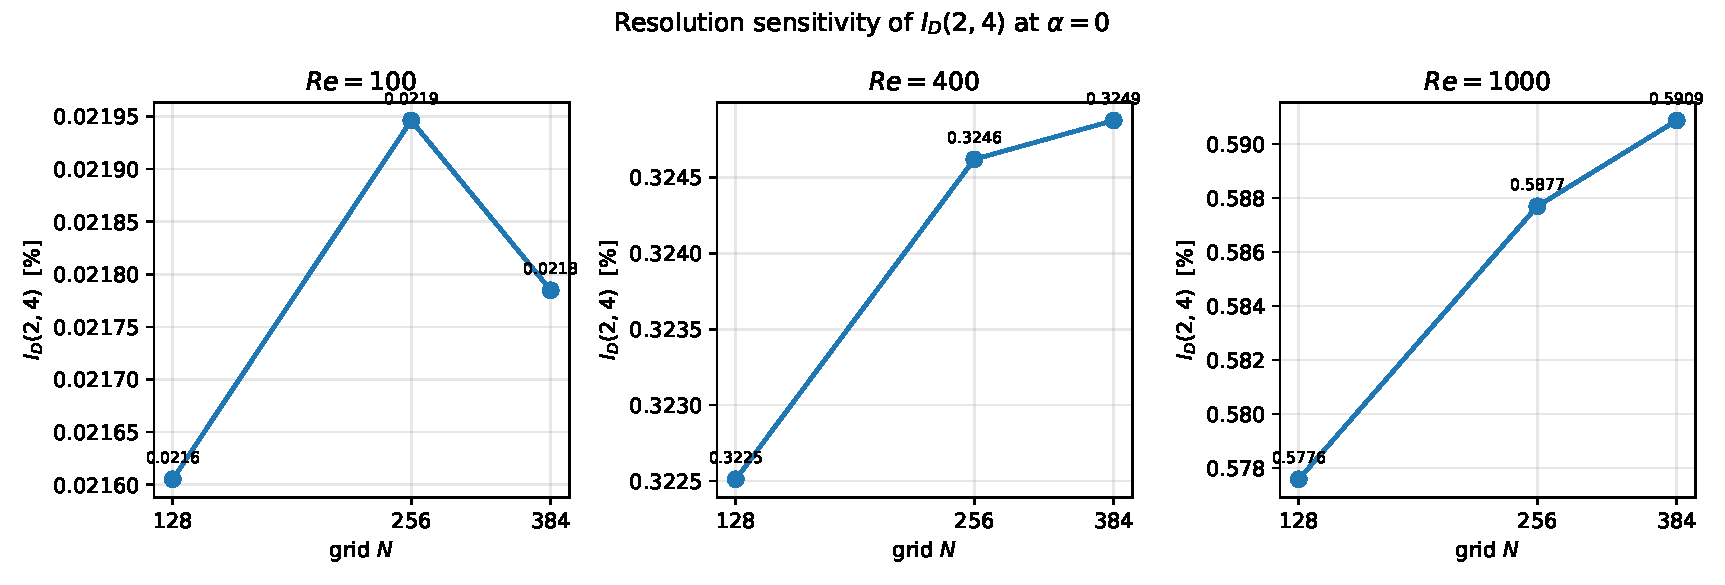
\includegraphics[width=0.95\columnwidth]{figures/fig6_resolution.pdf}
\caption{(Color online) Resolution sensitivity of the primary contrast $I_D(2,4)$ at $\alpha=0$. Panels: (a) $Re=100$; (b) $Re=400$; (c) $Re=1000$. The contrast is stable to better than $1\%$ between $N=256$ and $N=384$ at all Reynolds numbers; the full $N = 128$--$384$ spans quoted in the text are the conservative numerical uncertainties on $I_D(2,4)$ used throughout.}
\label{fig:resolution}
\end{figure}

\subsection{Reynolds-number dependence of the primary contrast}
\label{subsec:redependence}

To explore the continuous variation with Reynolds number, an exploratory parameter sweep was performed at $N=128$ ($Re$ from $100$ to $1000$ in steps of $50$, all $n$ and both amplitudes; complete LBM parameters tabulated in Table~SM.III of the Supplemental Material). Because this exploratory sweep is conducted on a relatively coarse mesh where the lattice Mach number reaches $Ma\approx0.18$ at higher $Re$, its quantitative details must be distinguished from the primary contrast $I_D(2,4)$ established at $N=384$ ($Ma\le0.06$) across the three benchmark Reynolds numbers. The sweep serves a descriptive purpose: it resolves how the contrast transitions from low to moderate Reynolds numbers. The contrast grows monotonically from $0.022\%$ at $Re=100$ to $0.578\%$ at $Re=1000$. Its local logarithmic slope $\gamma_{\rm loc}=d\ln|I_D|/d\ln Re$, evaluated by central differences, \emph{decreases} steadily from $2.72$ near $Re=150$ to $0.47$ near $Re=950$, crossing unity near $Re\approx346$ (Fig.~\ref{fig:resweep}b). The contrast therefore grows \emph{super}-linearly ($\gamma_{\rm loc}>1$) below $Re\approx346$ and \emph{sub}-linearly ($\gamma_{\rm loc}<1$, approaching a $\sqrt{Re}$-like behaviour) above it; the transition between the two regimes is a smooth, monotone decrease of $\gamma_{\rm loc}$ through unity rather than a sharp break. The two terms of the partition of Section~\ref{subsec:mechanism} provide a quantitative account of this: along the same $N=128$ sweep, the added-region term $dB$ grows nearly linearly in $Re$, whereas the common-region redistribution $\mathrm{d}A$ is negative at $Re=100$, crosses zero near $Re\approx145$, peaks near $Re\approx600$, and then declines (Table~SM.XIV of the Supplemental Material). Because the total is $dA+dB$, a contrast that is super-linear at low $Re$ (where $dA$ is rising fastest), flattens as $dA$ saturates, and becomes sub-linear at high $Re$ (where the linear $dB$ term dominates and $dA$ declines) follows from the two-term structure rather than from any single dominant region. This is the physical content of the crossover: the super-linear growth at low $Re$ is the signature of the common-region redistribution $\mathrm{d}A$ rising fastest, the flattening near $Re\approx346$ is where $\mathrm{d}A$ begins to saturate, and the sub-linear growth at high $Re$ is where the linear added-region term $\mathrm{d}B$ dominates and $\mathrm{d}A$ declines. The crossover is therefore not a fitted exponent but a direct consequence of the two-term structure of the partition. The contrast grows by a factor of about $15$ from $Re=100$ to $400$ but only by a factor of about $1.8$ from $Re=400$ to $1000$, tracking the passage of $\gamma_{\rm loc}$ through unity. We emphasize that the local slope $\gamma_{\rm loc}$ and the crossover at $Re\approx346$ are descriptive features of this coarse-grid trajectory, not universal scaling thresholds or grid-converged laws.

An independent, finer-grid sweep reinforces the same trend through a different observable. Evaluated at $N=256$ ($Ma\approx0.090$) over $Re=100$--$375$, the enstrophy contrast $Z_4-Z_2$, where $Z=\sum\omega^2\,\mathrm{d}A$ is the integrated squared vorticity, grows monotonically from $+0.005$ at $Re=100$ to $+0.074$ at $Re=375$---consistent with the dissipation-based growth above, but measured on a distinct quantity. Because $Z$ is enstrophy and not $D^*$, this sweep does not by itself extend $I_D(2,4)$ to the intermediate Reynolds numbers; doing so requires the same sweep to be re-evaluated with the dissipation estimator, which we leave for follow-up work.

\begin{figure}[t]
\centering
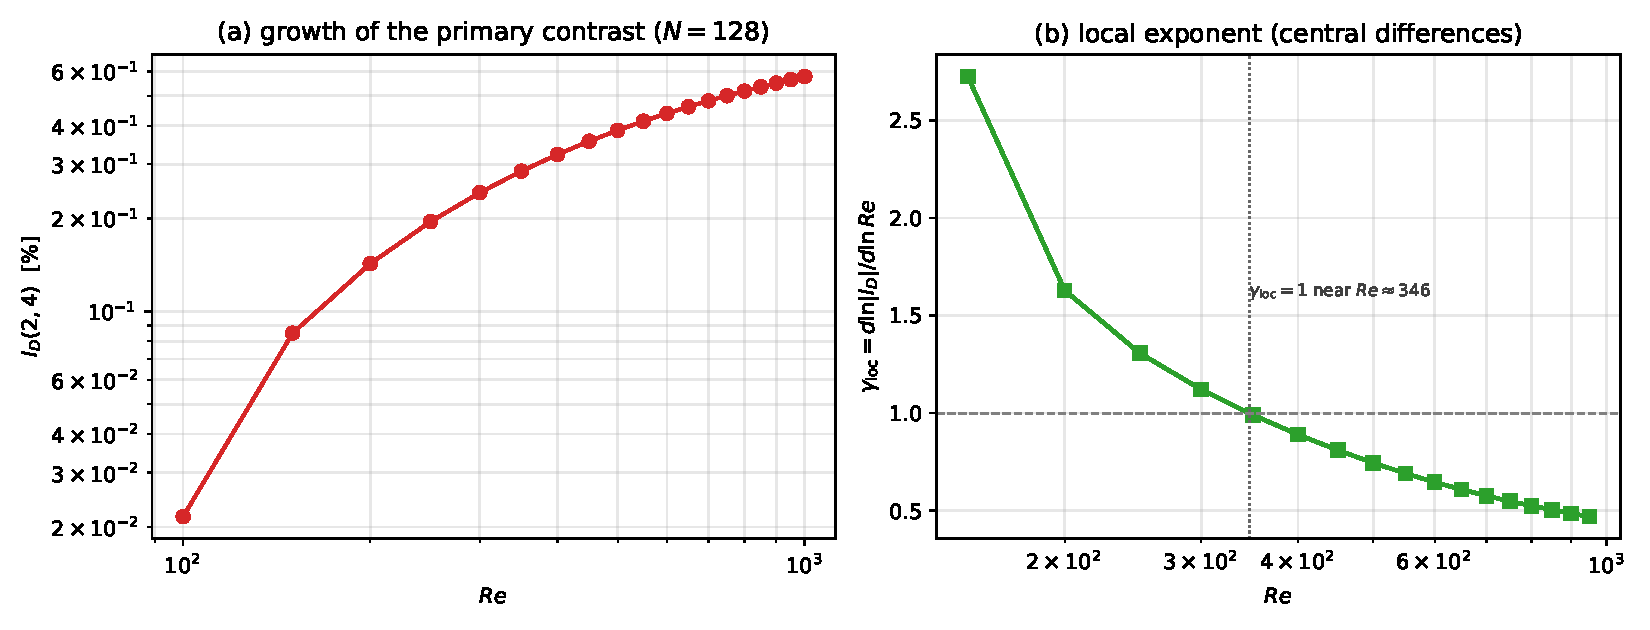
\includegraphics[width=0.98\columnwidth]{figures/fig9_resweep.pdf}
\caption{(Color online) Reynolds-number dependence of the primary contrast $I_D(2,4)$ at $\alpha=0$ from the $N=128$ sweep. (a) log--log growth from $Re=100$ to $1000$. (b) Local exponent $\gamma_{\rm loc}=d\ln|I_D|/d\ln Re$ (central differences), which falls smoothly through unity near $Re\approx346$. The local slope decreases through unity over this exploratory sweep, indicating a transition from superlinear to sublinear growth; these slopes are descriptive and do not establish a universal scaling law.}
\label{fig:resweep}
\end{figure}

\subsection{Robustness of the contrast}
\label{subsec:robustness}

The small magnitude of the contrast makes it essential to show that it is not an artifact of a single numerical choice. We report three independent tests, all at $N=384$ and $\alpha=0$.

\emph{(i) Wall-gradient treatment.} Recomputing the local strain rate with a purely one-sided node-based bottom-wall gradient, instead of the geometric wall-distance correction used in the reference diagnostics, changes $I_D(2,4)$ from $0.0218\%$ to $0.0207\%$ ($Re=100$, a relative change of $5.0\%$), from $0.3249\%$ to $0.3212\%$ ($Re=400$, $1.1\%$), and from $0.5909\%$ to $0.5777\%$ ($Re=1000$, $2.2\%$). The contrast therefore survives the change of wall treatment to within a few percent of its own value; the largest relative sensitivity is at $Re=100$, where the absolute contrast is smallest, while at $Re=400$ and $1000$ the change is $1$--$2\%$.

\emph{(ii) Geometry-dependent effective Reynolds number.} Flattening the bottom changes the flow depth, so the effective Reynolds number felt by the flow differs slightly between the two geometries; an upper bound of $0.4\%$ on this difference (the relative change of the characteristic depth between $n=2$ and $n=4$ times the $Re$ sensitivity) propagates, through the slope $dI_D/dRe$ measured in Section~\ref{subsec:redependence}, to a change of $0.0005\%$ in $I_D(2,4)$ at $Re=100$ (about $2\%$ of its value) and $0.0011\%$ at $Re=400$ (about $0.4\%$). The contrast is dominated by the geometry at fixed $Re$, not by the small $Re_{\rm eff}$ drift.

\emph{(iii) Resolution.} As reported in Section~\ref{subsec:resolution}, $I_D(2,4)$ is stable to within a few percent of its value over the full $N=128$--$384$ range; the absolute integrals are not, and carry a residual grid dependence of order $1\%$. The refinement ratios are not uniform and the residual change between the two finest grids is not a clean power-law decay, so no Richardson extrapolation or grid-convergence index is reported. Instead the observed span of $I_D(2,4)$ over $N=128$--$384$ is retained as the conservative numerical uncertainty: $3.4\times10^{-4}$ percentage points ($Re=100$), $2.4\times10^{-3}$ ($Re=400$), and $1.3\times10^{-2}$ ($Re=1000$), i.e.\ at most $2.3\%$ of the finest-grid contrast. The extrapolated values are not used; the $N=384$ values are quoted throughout, with this span as their resolution uncertainty.

The three tests are mutually consistent and bound the contrast to be robust to wall treatment, to the effective-Reynolds drift, and to resolution, at the level of a few percent of its own value. An independent finite-element (Taylor--Hood) solution was additionally used to cross-validate the LBM bulk solver, both on the benchmark cavity (Section~\ref{subsec:validation}) and, on the superelliptic family, at the level of the primary contrast itself. All finite-element energetics are native (element-wise integrals, no projection), and their energy balance closes to $0.01\%$ on $nx=256$ (and within $0.22\%$ over all meshes, contrasting with the $\approx 2\%$ LBM shear-layer defect). On three meshes ($nx=64/128/256$) the finite-element dissipation contrast is $I_D(2,4)=+0.346\%,+0.332\%,+0.323\%$, and the finest-mesh value $+0.323\%$ lies $0.002$ percentage point from the lattice-Boltzmann value $+0.325\%$ at $N=384$; on the matched finest grids (FEM $nx=256$, LBM $N=384$) all three contrasts agree to within $0.02$ percentage point, and the absolute levels agree to $1$--$4\%$ (Section~\ref{subsec:validation} and the supplementary material). Because the finite-element variation across its own meshes exceeds the final FEM--LBM gap, this is a cross-solver consistency check for the contrast rather than an independent convergence result. A broader cross-solver sweep over the full parameter matrix remains a follow-up.

\subsection{Energetic consistency and estimator agreement}
\label{subsec:consistency}

Two distinct diagnostics are reported. First, the global energy balance of each simulation: the signed relative imbalance $(P^*-D^*)/D^*$ is negative in every case, with magnitude about $2\%$ at $N=384$ ($1.98\%$ at $Re=100$, $2.04\%$ at $Re=400$, $2.13\%$ at $Re=1000$). This residual is not a constant; it decreases with grid refinement as a first-order (in $1/N$) discretisation error, from $-6.2\%$ at $N=128$ to $-2.0\%$ at $N=384$ at $Re=400$ (Section~VII.A of the Supplemental Material). It is therefore a resolution-limited defect of the absolute integrals, not a fixed offset between the lid momentum-exchange estimator of $P$ and the strain-rate estimator of $D$. Second, the agreement between the power-based and dissipation-based estimates of the same matched contrast, $\delta_{IP/ID}=100|I_P/I_D-1|$. For the dominant transition $(2,4)$ at $\alpha=0$, the values are $3.1\%$ ($Re=100$), $1.0\%$ ($Re=400$), and $1.9\%$ ($Re=1000$): the two independent routes to the contrast agree to a few percent at $N=384$.

The agreement degrades for the weaker transitions: at $Re=400$, $\delta_{IP/ID}$ is $10.3\%$ for $(4,6)$ and undefined in any meaningful sense for $(6,8)$, where both $I_P$ and $I_D$ are at the level of $10^{-4}\%$ and their ratio is dominated by cancellation. This degradation is expected: a small difference of two large numbers is sensitive to the small systematic offset between the $P$ and $D$ estimators. It is therefore the dominant $(2,4)$ contrast, not the weak higher-order transitions, that supports a quantitative consistency statement. The reason the contrast is stable even though the absolute defect is not is that, at fixed $(\tau,U)$, the $n = 2$ and $n = 4$ states carry the same leading-order discretization and compressibility defect, which therefore cancels to first order in the paired difference. This is demonstrated, not assumed, by the grid $\times$ Mach factorial of Table~SM.IV: at $Re = 400$ a factor-eight change of $Ma$ moves the absolute defect by $2.0$ points at $N = 128$ (from $-4.24\%$ to $-6.25\%$) but moves $I_D(2,4)$ by only $0.0019$ point, i.e.\ by about $0.6\%$ of its own value. Crucially, this estimator agreement does not replace the resolution analysis: the two estimators may agree well at a given $N$ while both still carry a common grid error. The resolution study of Section~\ref{subsec:resolution} remains the relevant test of grid sensitivity.

\subsection{Influence of the undulation amplitude and integration}
\label{subsec:amplitude}

The amplitude $\alpha$ has two effects. First, it reduces the fluid area at fixed $n$ (by about $5.6\%$ from $\alpha=0$ to $0.1$ at $n=2$) and produces a corresponding uniform downward shift of $P^*$ and $D^*$ (Fig.~\ref{fig:energetic}). Second, and more importantly, it modifies the magnitude of the geometric contrast itself. At $Re=400$ the $(2,4)$ contrast falls from $+0.325\%$ at $\alpha=0$ to $+0.133\%$ at $\alpha=0.1$; at $Re=1000$ it falls from $+0.591\%$ to $+0.078\%$; at $Re=100$ it falls from $+0.022\%$ to $+0.008\%$. This is a genuine interaction in the sense of Section~\ref{subsec:interaction}: the change in the contrast produced by increasing $n$ depends on the undulation amplitude. In percentage points, the interaction for $(2,4)$ at $Re=400$ is $-0.19$, i.e.\ the contrast at $\alpha=0.1$ is about $0.19$ percentage points smaller than at $\alpha=0$. The hierarchy remains qualitatively the same at both amplitudes, but its quantitative strength is amplitude-dependent, and the contrast is weaker when the wall is undulated.

At $Re=1000$ and $\alpha=0.1$ the sign structure itself changes: while $(2,4)$ is still positive at this amplitude ($+0.0782\%$), both $(4,6)$ and $(6,8)$ become negative ($-0.0242\%$ and $-0.0052\%$). The interaction between $n$ and $\alpha$ is therefore not only quantitative (weaker contrast) but also qualitative (sign reversal of the trailing transitions). That reversal is not exclusive to the highest Reynolds number: at $\alpha=0.1$ and $Re=400$ the same two transitions are already negative ($-0.0039\%$ and $-0.0017\%$), each larger in magnitude than its own $N=128$--$384$ span. Undulating the wall thus flips the sign of the trailing transitions at both Reynolds numbers, and increasing $Re$ amplifies the effect; at the flat wall ($\alpha=0$), by contrast, the sign of the $(6,8)$ transition is itself a Reynolds-dependent feature---positive and resolved at $Re=100$ ($+0.00042\%$, $5.2$ times its own span), unresolved at $Re=400$, negative and resolved at $Re=1000$.

Taken together, the three levels of the analysis are coherent. The flow fields change only moderately with geometry; the integrated dissipation changes by a small fraction of a percent despite an area change of several percent; and the contrast hierarchy is stable across Reynolds numbers, resolutions, and amplitudes while its magnitude depends on both $Re$ and $\alpha$. The dominant uncertainty is the residual grid dependence of the absolute integrals (about $1\%$), not the stability of the contrasts themselves.

\subsection{Scope and limitations}
\label{subsec:scope}

The results above establish the robustness of the paired contrasts, not the grid-independence of the absolute integrals. We collect here the limits of the present study. (i) No Richardson extrapolation or grid-convergence index is reported, because the refinement ratios are not uniform and the residual change between the two finest grids is dominated by partial cancellation of common discretisation error rather than by a clean power-law decay; the span of $I_D(2,4)$ over $N=128$--$512$ is retained as the conservative numerical uncertainty. (ii) The absolute integrals carry a residual grid dependence of order $1\%$ between $N=256$ and $N=384$; no claim of grid-independent absolute energetics is made. (iii) The Taylor--Hood finite-element comparison is a cross-solver consistency check, not a convergence proof for either solver, because the finite-element variation across its own meshes exceeds the FEM--LBM gap. (iv) The scope is limited to the tested superellipse family, single undulation count $N_w=1$, and the three Reynolds numbers studied; the unmatched Mach numbers of the coarse $n\ge6$ runs at $Re=100$ preclude any claim that the trailing-transition signs at $Re=100$ are grid-converged. (v) The $N=512$ extension is available only at $Re=400$ and $Re=1000$, $\alpha=0$; it confirms the stability of the primary contrast (to within $3\times10^{-5}$~pp between $N=384$ and $N=512$ at $Re=400$) and strengthens the negative sign of the $(6,8)$ transition at $Re=1000$, but does not alter the qualitative conclusions drawn from the $N=128$--$384$ sequence.

Table~\ref{tab:claims_evidence} collects the main claims of this study, the evidence on which each rests, and the associated uncertainty. The purpose is to make explicit which conclusions are resolution-backed and which remain qualitative or partial.

\begin{table*}[!htbp]
\centering
\caption{Summary of claims, evidence, and uncertainties. Each row pairs a central statement with the data that support it and the resolution or modeling limitation that bounds its interpretation. ``Resolved'' indicates whether the claim is backed by a contrast whose magnitude exceeds its own $N=128$--$512$ span.}
\label{tab:claims_evidence}
\resizebox{\textwidth}{!}{%
\begin{tabular}{@{}llll@{}}
\hline
\textbf{Claim} & \textbf{Evidence} & \textbf{Uncertainty} & \textbf{Resolved?} \\
\hline
$I_D(2,4)>0$ at $Re=100,400,1000$ & $N=384$ values; spans & $3.4\times10^{-4}$, $2.4\times10^{-3}$, $1.4\times10^{-2}$~pp & Yes \\
Hierarchy $|I(2,4)|\gg|I(4,6)|\gg|I(6,8)|$ & $N=384$ + per-transition spans & Own spans per transition & Yes at $Re=400,1000$; partial at $Re=100$ \\
$\mathrm{d}B>0$ at all $Re$ & four bands at $N=128$--$512$ (Table~SM.XV) & positive on every grid; magnitude $\le3\%$ span & Yes (sign) \\
$\mathrm{d}A$ changes sign near $Re\approx145$ & four bands at $N=128$--$512$ (Table~SM.XV) & sign stable across grids; magnitude up to $27\%$ at $Re=1000$ & Yes (sign) \\
Sub-extensivity (factor 13--364) & $I_D$ vs $I_{D,\text{area}}$ & Dominated by $I_D$ uncertainty & Yes \\
FEM--LBM cross-solver consistency & $nx=256$ vs $N=384$ & 0.002--0.008~pp & Consistency only \\
\hline
\end{tabular}%
}
\end{table*}









